\chapter{Method}

My special method. 

\section{Architecture}

\subsection {Convolution layer}

A convolution layer takes \textit{n} images as input, $ I_1, I_2, \dots, I_n $, and produces \textit{m} intermediate outputs, $O_1, O_2, \dots, O_m $. It also contains \textit{m} kernels, $ K_1, K_2, \dots, K_m $. Each kernel $ K_i $ is convolved with all the input images, and each respective pixel from each convolution is then summed, added a bias to, and sent through a non-linear function. Afterwards the resulting matrix is subsampled/max-pooled, where it is divided into $ p \times p $ non-overlapping neighborhoods, from which the maximum value is extracted. The result of the max-pool operation the output image $ O_i $. 
In the first layer of the network there is only one input image (i.e. $ n = 1 $), thus no summation is needed. 

The overall architecture of the convolution layer is separated into four modules. A convolution module, a summation buffer, a non-linear function module and a subsample/max-pool module.

\vspace*{1\baselineskip}
\textbf{The convolution module} (CM) is inspired by \cite{Farabet2009}. The input is a $ n \times n $ image \textit{I}, and the output is a $ (n-k+1) \times (n-k+1) $ convolved image \textit{C}, using a $ k \times k $ kernel \textit{K}. Every clock cycle the module takes in a pixel as input, and after a certain delay it will output a processed pixel almost every cycle. Each pixel is inputted once, left to right, one row at a time. 

\begin{figure}[h!]
  \centering
      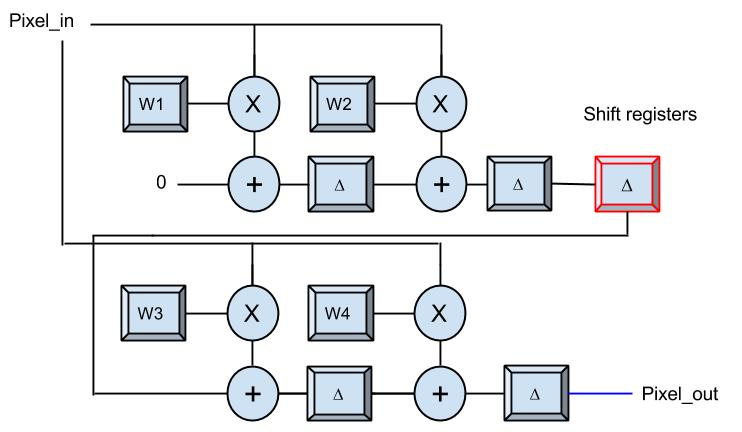
\includegraphics[width=1.0\textwidth]{Figures/Method/Convolver}
  \caption{The convolution module, when $ n = 3 $ and $ k = 2 $.}
\end{figure}

It consists of 2D grid of multiply and accumulate (MAC) units which represents the convolution kernel. Thus the grid dimension is equal to the kernel dimension. In every MAC unit there is a register that contains the respective kernel weight. In every clock cycle the MAC units multiply the input pixel with its weight, and then accumulates the result from the previous cycle of the MAC unit to the left. 

At the end of each row of MACs there is $ n - k $ shift registers. The result of the last MAC in each row is stored in the first shift register, and the first MAC in each row takes the value of the last shift register of the previous row as accumulation input. The exception being the absolute first and last MAC unit. Every clock cycle the values in the shift registers are shifted to the right. 
	
By providing this delay you only have to input each pixel once during the convolution. Generally every pixel is needed for $ k \times k $ convolution operations (the exception being the pixels close to the boarders of the image). Thus the shift registers are used to store the intermediate values of the convolutions until a pixel that is needed for the respective convolution operation is inputted. 

The delay these shift registers cause are the reason for the delay before valid output pixels are produced. Thus from when the convolution starts, the output will not be valid before $ k-1 $ rows of the image have been processed. And for every new image row, there will be a $ k-1 $ cycle delay before output is valid. This is demonstrated by the fact that the input image is a $ n \times n $matrix, while the output matrix is a $ (n-k+1) \times (n-k+1) $ matrix. 

The loading of the weights takes $ k \times k $ clock cycles, and the processing of the image takes $ n \times n $ clock cycles. Thus the total number of cycles it takes to perform a full convolution of an image is $ n \times n + k \times k $. But \textit{n} tends to be larger than \textit{k}. e.g. $ n = 32 $ and $ k = 5 $is a fairly normal problem size (FIND SOURCES FOR THIS!), which makes the weight loading take 25 clock cycles and the image processing 1024 cycles. This means that the execution time of the CM is mostly bounded by the size of the image. Though it is important to note that the CM is resource expensive, in that it requires $ k \times k $ DSP slices on the FPGA.

\begin{figure}[h!]
  \centering
      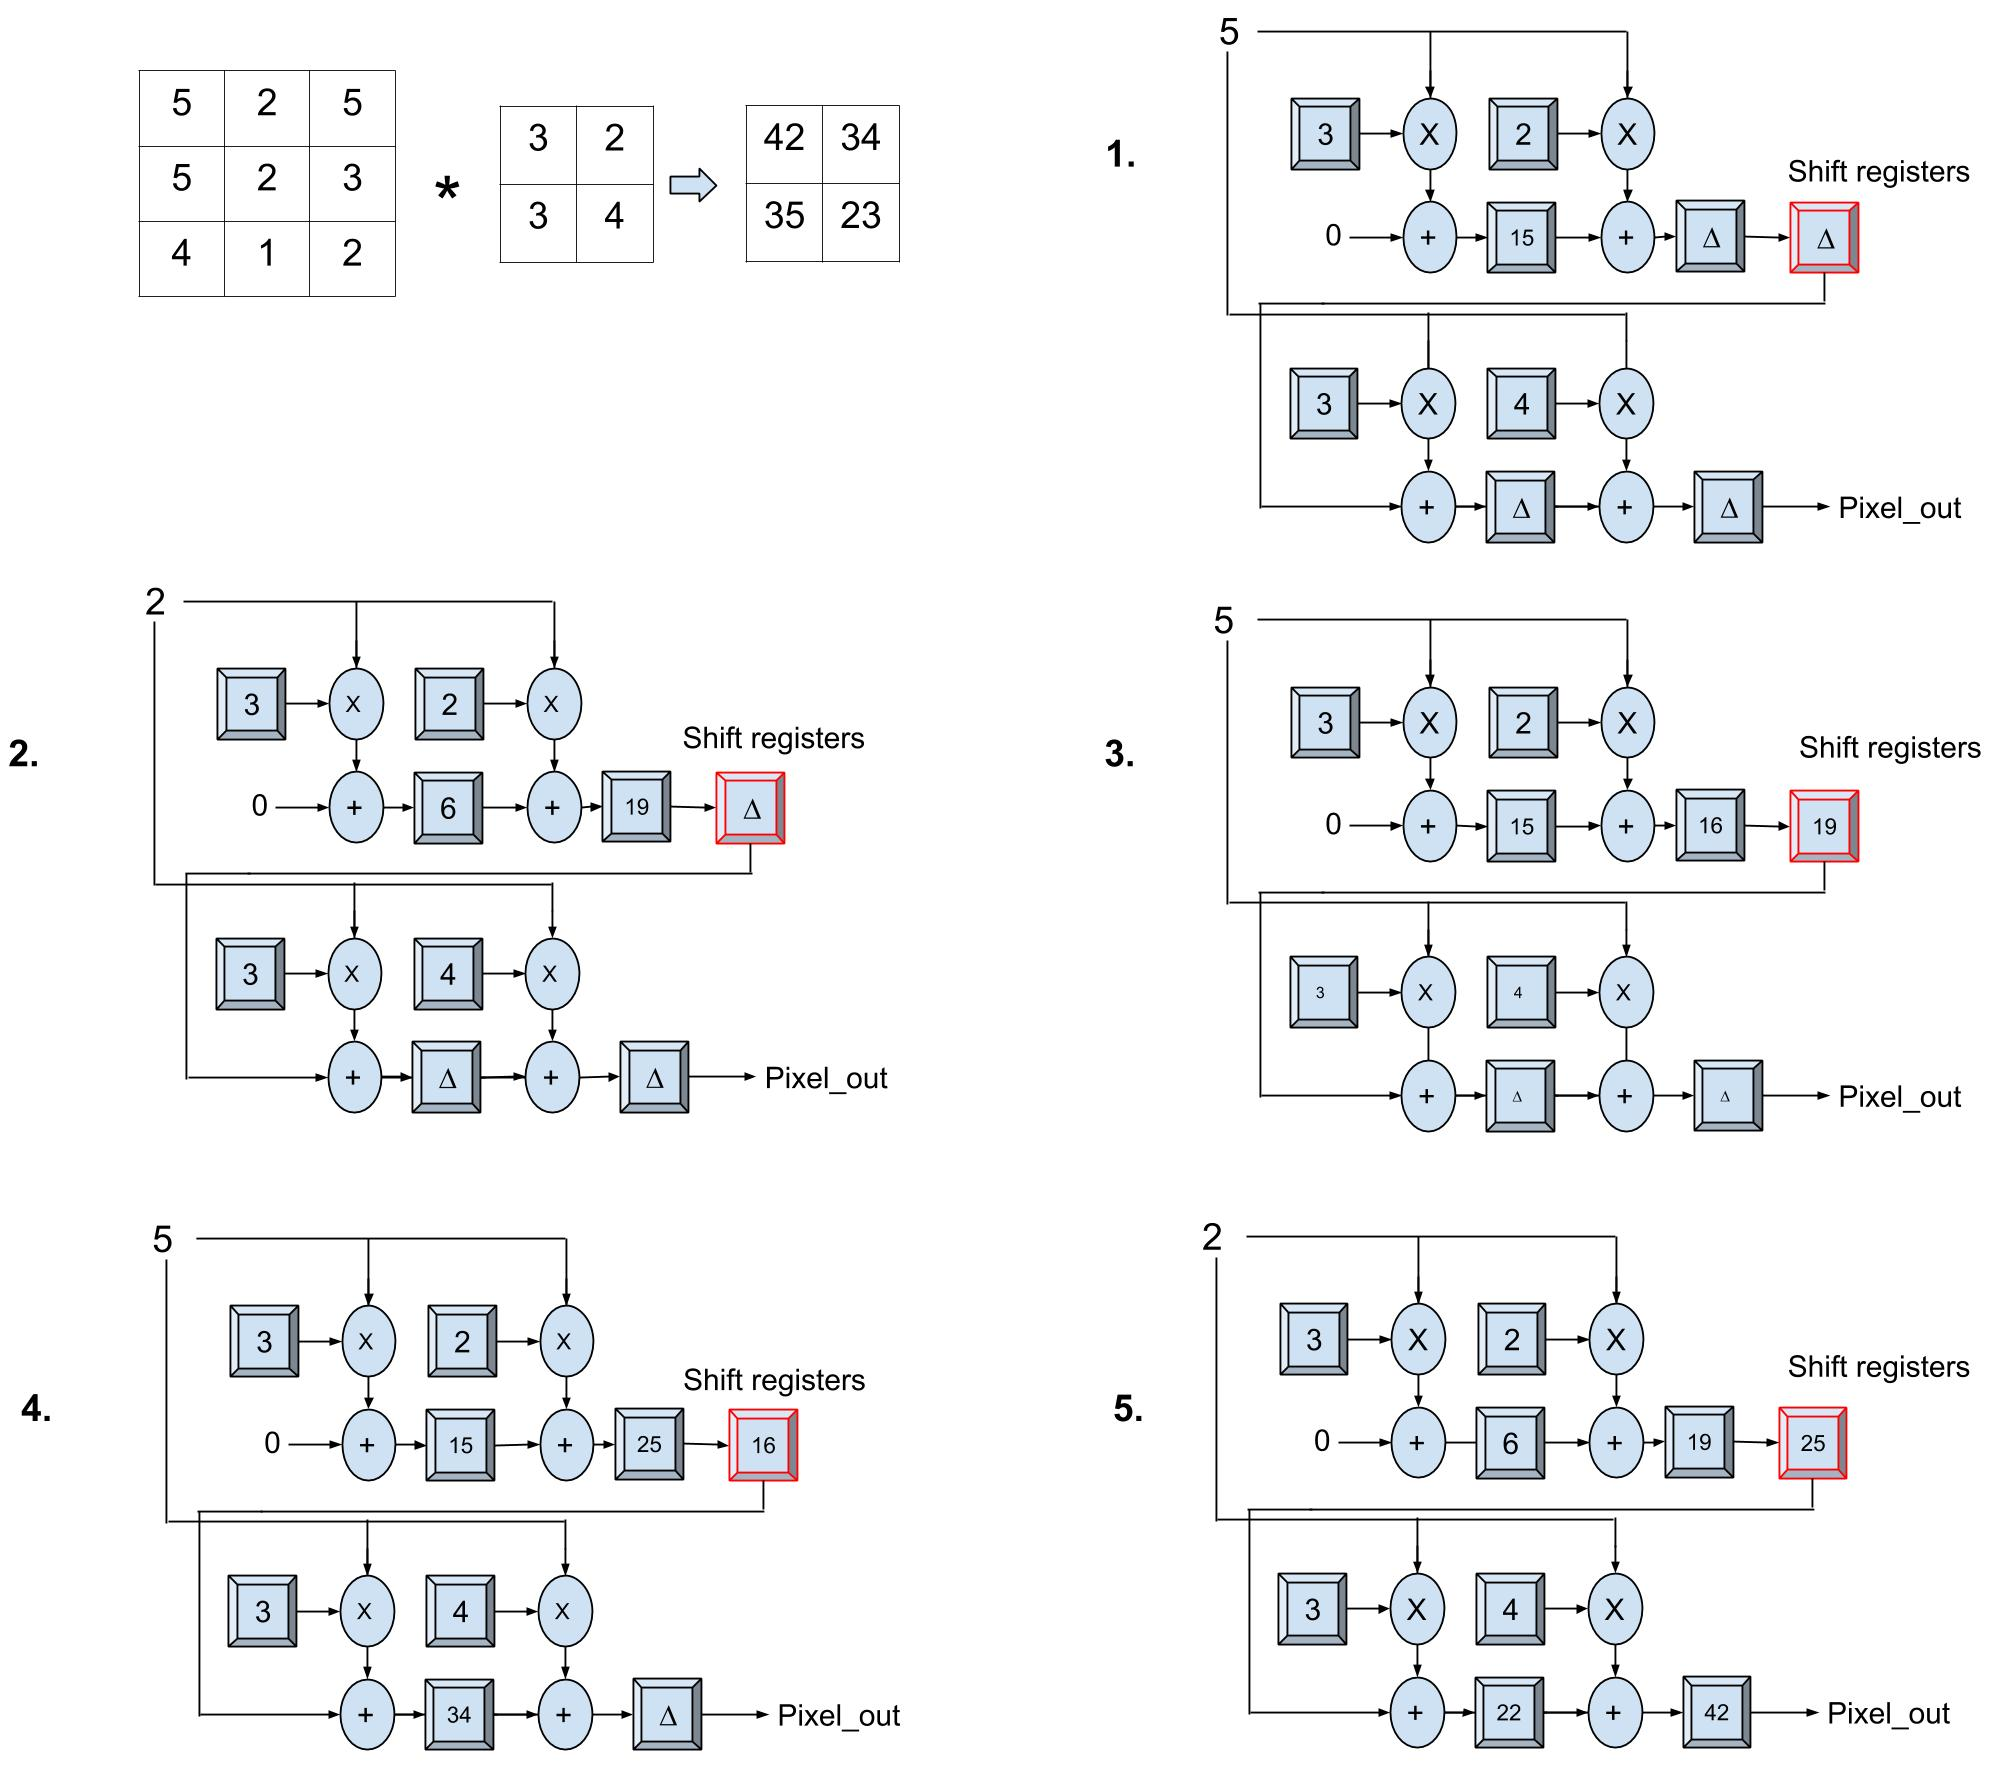
\includegraphics[width=1.0\textwidth]{Figures/Method/Conv_example}
  \caption{Example showing the five first clock cycle of an convolution. ADD IMAGE SHOWING THE EXAMPLE MATRICES!}
\end{figure}

\vspace*{1\baselineskip}
REWRITE FIRST PART
\textbf{The subsample/max-pooling module} (SS/MP) was designed to complement the CM and avoid being a bottleneck. Thus it was designed to act in the same streaming way as the convolution module, and be done processing at almost the same time. The input is a $ (n-k+1) \times (n-k+1) $ convolved image \textit{C}, and the output is a $ (n-k+1)/p \times (n-k+1)/p $ SS/MP image \textit{P}, where \textit{p} is the dimension of subsample neighborhood. As with the CM, one pixel is streamed in every cycle, and streamed out whenever a valid pixel is ready. Designed this way the SS/MP can process in parallel with the CM, by directly streaming the output of the CM into the SS/MP module. 

The module consist of a module which compares the input with the current max value, and updates the max value accordingly. It also contains a set of \textit{(n-k+1)/p} shift registers. Since the image is divided into $ p \times p $ non-overlapping neighborhoods, the module needs to store the current maximum value of previous neighborhood when a pixel from a new neighborhood is inputted. To do this the module contains counters, \textit{row\_num} and \textit{column\_num}. When a new pixel is inputted the \textit{column\_num} counter is incremented, and when a new row is encountered the \textit{row\_num} counter is incremented. Every time $ column_num mod p = 0 $ the shift registers are shifted one to the right, and every time $ column_num mod p = 0 and row_num mod p = 0 $ a valid output is produced. 

The execution speed of the SS/MP module is bounded by the size of the input image, $ c \times c $ clock cycles, finishing one cycle after the last pixel has been inputted. 
Thus by streaming the output of the CM to the SS/MP, both will finish only a few cycles apart, effectively running both jobs in parallel. The resource usage of the module is bounded by the size of the subsampling dimension, since it requires a number of shift registers equal to the size of the dimension. 